
\section{The Cumulus System}
\label{sec:architecture}


\subsection{Architecture}


\begin{figure}
\begin{center}
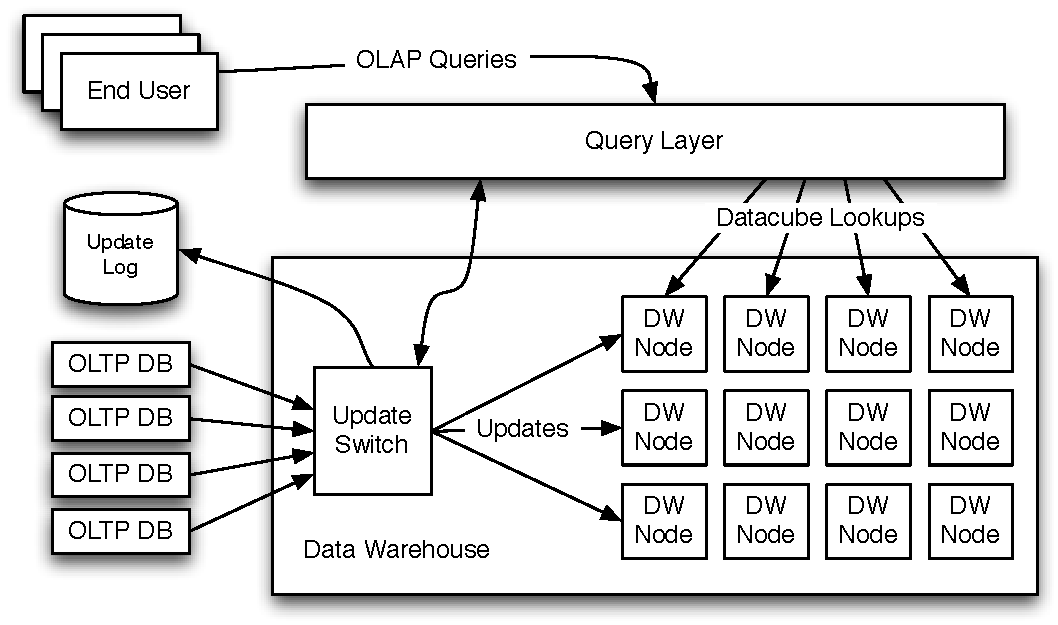
\includegraphics[width=3in]{images/Architecture.pdf}
\caption{Cumulus' architecture.}
\label{fig:arch}
\end{center}
\end{figure}


Cumulus consists of three components: a {\em runtime}, a {\em query layer},
and a compiler.  A diagram of this architecture is presented in Figure \ref{fig:arch}.  The warehousing runtime accepts updates -- insertions and deletes of tuples -- at a coordinator node called the \textit{Switch}, which delegates update work to an array of data warehouse storage and query processing nodes, or \textit{DW Nodes}.  For simplicity, we first present the system as if there is a single centralized switch, and explain a distributed switch implementation later, in Section \ref{sec:distswitch}.

The query layer of Cumulus acts as an intermediary between the users
and the DW nodes.  The query layer accepts roll-up/drill-down/slice/dice
queries, translates them into the corresponding set of data warehouse
lookups, and creates a query result from the data returned.
%
% The Query Layer is
% implemented in a client-side API that runs on the user machines.

Cumulus' final component is the compiler, which was discussed in the
previous section. The compiler translates SQL aggregation queries
into message passing programs that are executed by the switch and the DW nodes.
The maps suggested by the compiler -- and maintained by the M3 program --
are partitioned across the DW nodes to keep network traffic to a minimum.  


This section is structured as follows. We first give a description of
the meaning of message passing programs in the context of distributed
evaluation. Then we discuss the protocol for message passing, and the role
of the switch in update processing. Next, we explain how our protocol, and
the design of switch and DW nodes, guarantees consistency of the
map datastructures. Finally, we discuss distributing the switch.


\subsection{Anatomy of an Update}


When a tuple is added to or removed from an input relation, the Switch
composes a set of messages parametrized on the tuple's contents and
dispatches them to the DW nodes as a sequence of map reads and writes.
Nodes being read from accept and process the requests and forward the
responses to the appropriate writers.  We refer to this entire sequence
of operations as an update.
The update corresponding to an M3 statement is coordinated by the subset of
nodes that store partitions of the map being written to.  Each node
coordinates updates only for those partitions it stores locally.
Simultaneously, read requests are dispatched by the switch to a subset
of the nodes managing partitions of the maps being read from, and the
responses are forwarded to the appropriate nodes managing the map to be
written to.  


\begin{figure}
\begin{center}
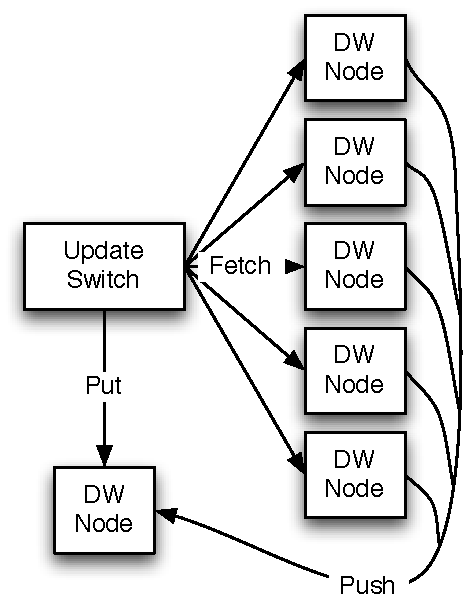
\includegraphics[width=1.5in]{images/UpdateStep.pdf}
\caption{Information flow during one map update.}
\label{fig:updatestep}
\end{center}
\end{figure}


A map update begins at the Switch when an input table is modified.  Each input table is associated with one or more triggers, each requiring a write to some range of map values and zero or more reads from different maps.  For each trigger, the Switch identifies and sends a PUT message to each DW node managing a map being written to.  Additionally, the Switch identifies all DW nodes managing maps that will be read from and sends a FETCH message to them, requesting the desired map values.  Finally, if required,
%
% (i.e., if Cumulus is being used standalone, without an underlying database),
%
the switch can log the update to disk for persistence.

The nodes receiving a FETCH request perform the appropriate reads and send their responses to the PUT nodes in a PUSH message.  Upon receipt of all necessary PUSH messages, the PUT nodes compute the update expression and modify the affected maps.  An illustration of the complete message-passing process is presented in Figure \ref{fig:updatestep}.  

\subsubsection{Trigger Dispatch}
Maps are partitioned along dimensional axes when they grow beyond the capacity of a single node, akin to the partitioning done in grid files\cite{318586}.  To streamline the dispatch of messages to component nodes, the switch pre-generates a spatial index for each template\footnote{Elsewhere called map update statement. It is convenient to think of such a statement, particularly if it is of the {\tt foreach} form, as a template of message passing.}, similar to the grid file directory.  Every entry in the spatial index contains a set of PUT and FETCH messages.  When the template is triggered, the tuple's values are used to index into the spatial index and the corresponding messages are parametrized and sent.  The algorithm for generating the spatial index is presented in Figure \ref{alg:dispatch}.

\begin{figure}
\begin{algorithmic}[1]
\STATE $Msgs \leftarrow \emptyset$
\FORALL{Update $U \in$ Trigger}
	\STATE Region $Reg = \pi_{U.target.loop\_vars} \left(index(U.target\_map)\right)$
	\FORALL{Partition $\{P | P\in U.target\_map \wedge (P \cap Reg \neq \emptyset)\}$}
		\STATE $Reads = \emptyset$
		\FORALL{Ref $R \in get\_map\_refs(U.expression)$}
			\STATE $RReg \leftarrow \pi_{R.loop\_vars} P$
			\STATE $RPart \leftarrow \{RP | RP\in R.map \wedge (RP \cap RReg \neq \emptyset)\}$
			\STATE $Reads \leftarrow Reads \cup \{(ReadP.node, R)\}$
		\ENDFOR
		\STATE $Reads \leftarrow group\_by\_node(Reads)$
		\STATE $Msgs \leftarrow put(U, P, Reads.size)$
		\FORALL{$($Node $N, \{$Ref $R\}) \in Reads$}
		  \STATE // PUSH results to $P.node$
			\STATE $Msgs \leftarrow fetch(N, \{R\}, P.node)$
		\ENDFOR
	\ENDFOR
\ENDFOR
\end{algorithmic}
\caption{The Switch's trigger dispatch algorithm}
\label{alg:dispatch}
\end{figure}

Looping updates require the Switch to match corresponding read and write partitions.  The correspondence is obtained by identifying intersections between partitions of the target map that are affected by the update, and those of each map in the update expression.  This is equivalent to a join over components of the spatial index stored at the Switch.  Loop-free updates are a special case of this, where only one partition is required from each map.  The trigger dispatch algorithm is shown in Figure \ref{alg:dispatch}.

\subsubsection{Get Collation}

FETCH responses, or PUSH messages for an update are sent to the node managing the partition being updated.  Having received the number of FETCH messages sent by the switch with the PUT message, the destination node can buffer PUSH messages until all have arrived.  At this point, if the update is loop-free, the destination node simply uses the contents of the PUSH messages to evaluate the update expression.

\begin{figure}
\begin{algorithmic}[1]
\STATE Given: Update $U$
\FORALL{Ref $R \in U.expression$}
	\STATE $Inputs \leftarrow Inputs \cup (R, \emptyset)$
\ENDFOR
\FORALL{$($Ref $InR,$ Value $V) \in \cup(msg_{PUSH})$}
	\FORALL{$(R, Table) \in Inputs$}
		\IF{$check\_match(InR, R)$}
			\STATE $Table \leftarrow Table \cup (InR.keys, V)$
		\ENDIF
	\ENDFOR
\ENDFOR
\FORALL{$(K,\{V\}) \in $ JOIN $ (Keys, Val) \in Inputs$}
	\STATE $Target = bind\_vars(U.target \leftarrow Keys)$
	\STATE $apply(Target, bind\_vars(U.expression \leftarrow \{V\}))$
\ENDFOR
\end{algorithmic}
\caption{The DW Node's collation algorithm}
\label{alg:collation}
\end{figure}

If the update requires a loop, the destination node must do some processing.  The node first generates a set of tables, one for each map reference in the update expression.  Arriving map values populate tables that correspond to any map reference matching the value's keys, where loop variables act as wildcards.  When all values have been received, the destination node computes the natural join of all of the generated tables, effectively producing one update value for every assigned value in the domain of all of the loop variables.  The loop-free update is a special case of this where each generated table contains only one row.  The collation algorithm is shown in Figure \ref{alg:collation}

\subsection{Update Consistency and Garbage Collection}

Cumulus' delta-encoding approach allows it to be agnostic to the order in which it processes input tuples.  However, this flexibility requires that an update's effect on the warehouse be logically atomic.  Atomicity is of particular importance, since the set of update rules triggered by a given update switch typically span the breadth of the data-dependency graph; Updates to any input relation typically have at least one read to a map updated by every other relation.

As the clearinghouse for updates, the Switch presents an ideal point for generating a total ordering over all tuples to be inserted into the warehouse.  The Switch maintains a version number for each node, incremented on every PUT dispatched to the node hosting it.  FETCHes sent to that node are tagged with the version number of the last PUT sent to the node, while PUTs are dependent on the completion of the prior PUT.

Data warehouse nodes ensure consistent evaluation of updates by buffering PUT requests received out of order, or prior to the completion of an earlier PUT request.  Similarly, FETCH requests for a particular version are buffered until the corresponding PUT request has completed, if it has not already done so.

Periodically, the switch queries each node for the completion status of pending PUT requests.  For each node, it computes the lowest FETCH version number for a read associated with an incomplete PUT request.  The Switch then disseminates these version numbers throughout the warehouse with a COMMIT message.  When a node receives a COMMIT, it snapshots its maps by discarding all updates for values that were overwritten before the commit version.


\subsection{Distributing the Switch}
\label{sec:distswitch}


The role of the switch is to provide a synchronization mechanism for the updates.  Specifically, the delta encoding approach used by the update rules requires that all update rules be applied to a consistent snapshot of the maps.  The current implementation of Cumulus performs this synchronization at a single node.  However, limiting the switch to only one node creates a scaling bottleneck.  

Despite the cloud computing mantra of rejecting consistency, this application requires it.  Complex locking protocols have poor scaling performance, so a simpler, lock-free protocol is required.  We achieve this goal by introducing the notion of \textit{pipeline scheduling}.  Pipeline scheduling exploits the acyclicity of compiler-generated data-flow graphs to allow nodes to correctly interleave and process update rules with only limited network overhead and processing latency.


{\em Pipeline Scheduling}.
Loose clock synchronization between nodes is assumed, and allows time to be partitioned into a sequence of numbered ticks, each lasting on the order of seconds.  When a set of updates is triggered, a switch node sends tentative put requests to all participating nodes.  These nodes respond with their current tick counter, and the switch forwards the maximum returned tick to all nodes.

The updates are considered to have been posted at the maximum returned tick.  However processing is deferred for a number of ticks equal to the depth of the map being updated.  The result is a data-flow process resembling a parallelized CPU pipeline.

During a given tick, all updates scheduled for processing are evaluated.  Once all updates scheduled for the tick have completed, the node responds to FETCH requests for the tick with PUSH messages.  Recall that each edge in the data flow graph represents a FETCH request for a specific update.  The difference in depth between the edge's ends is the number of ticks in advance of the PUT that the response is sent.  

For example, in Figure \ref{fig:dataflow} without removing any edges,
$Depth(q) = 2$, $Depth(qC) = 1$, and $Depth(qO2) = 0$.  Updates to map $q$ scheduled for processing during tick 4 would receive data from map $q_C$ during tick 3, and from map $q$ during tick 2.

